% !TeX root = ../report_project_2stage_OTA.tex

\section{Transistor-Level Design}

The ideal two-stage model is replaced by the complete SKY130A
transistor-level implementation. Device dimensions are first obtained
from the $g_m/I_D$ characterization, then refined using DC, AC, and
statistical simulations. The sequence is important: the first working
transistor-level circuit is a \emph{starting point}, not the final
sizing used for characterization in Section~6.

% RELEASE CHECK: Re-export this schematic from the FINAL Xschem design.
% The previously compiled PDF still showed NLOAD_0/1=0.6/2,
% NLOAD_2=0.6/2 (m=12), C_M=799.9 fF and R_M=110 kohm.
\begin{figure}[ht]
    \centering
    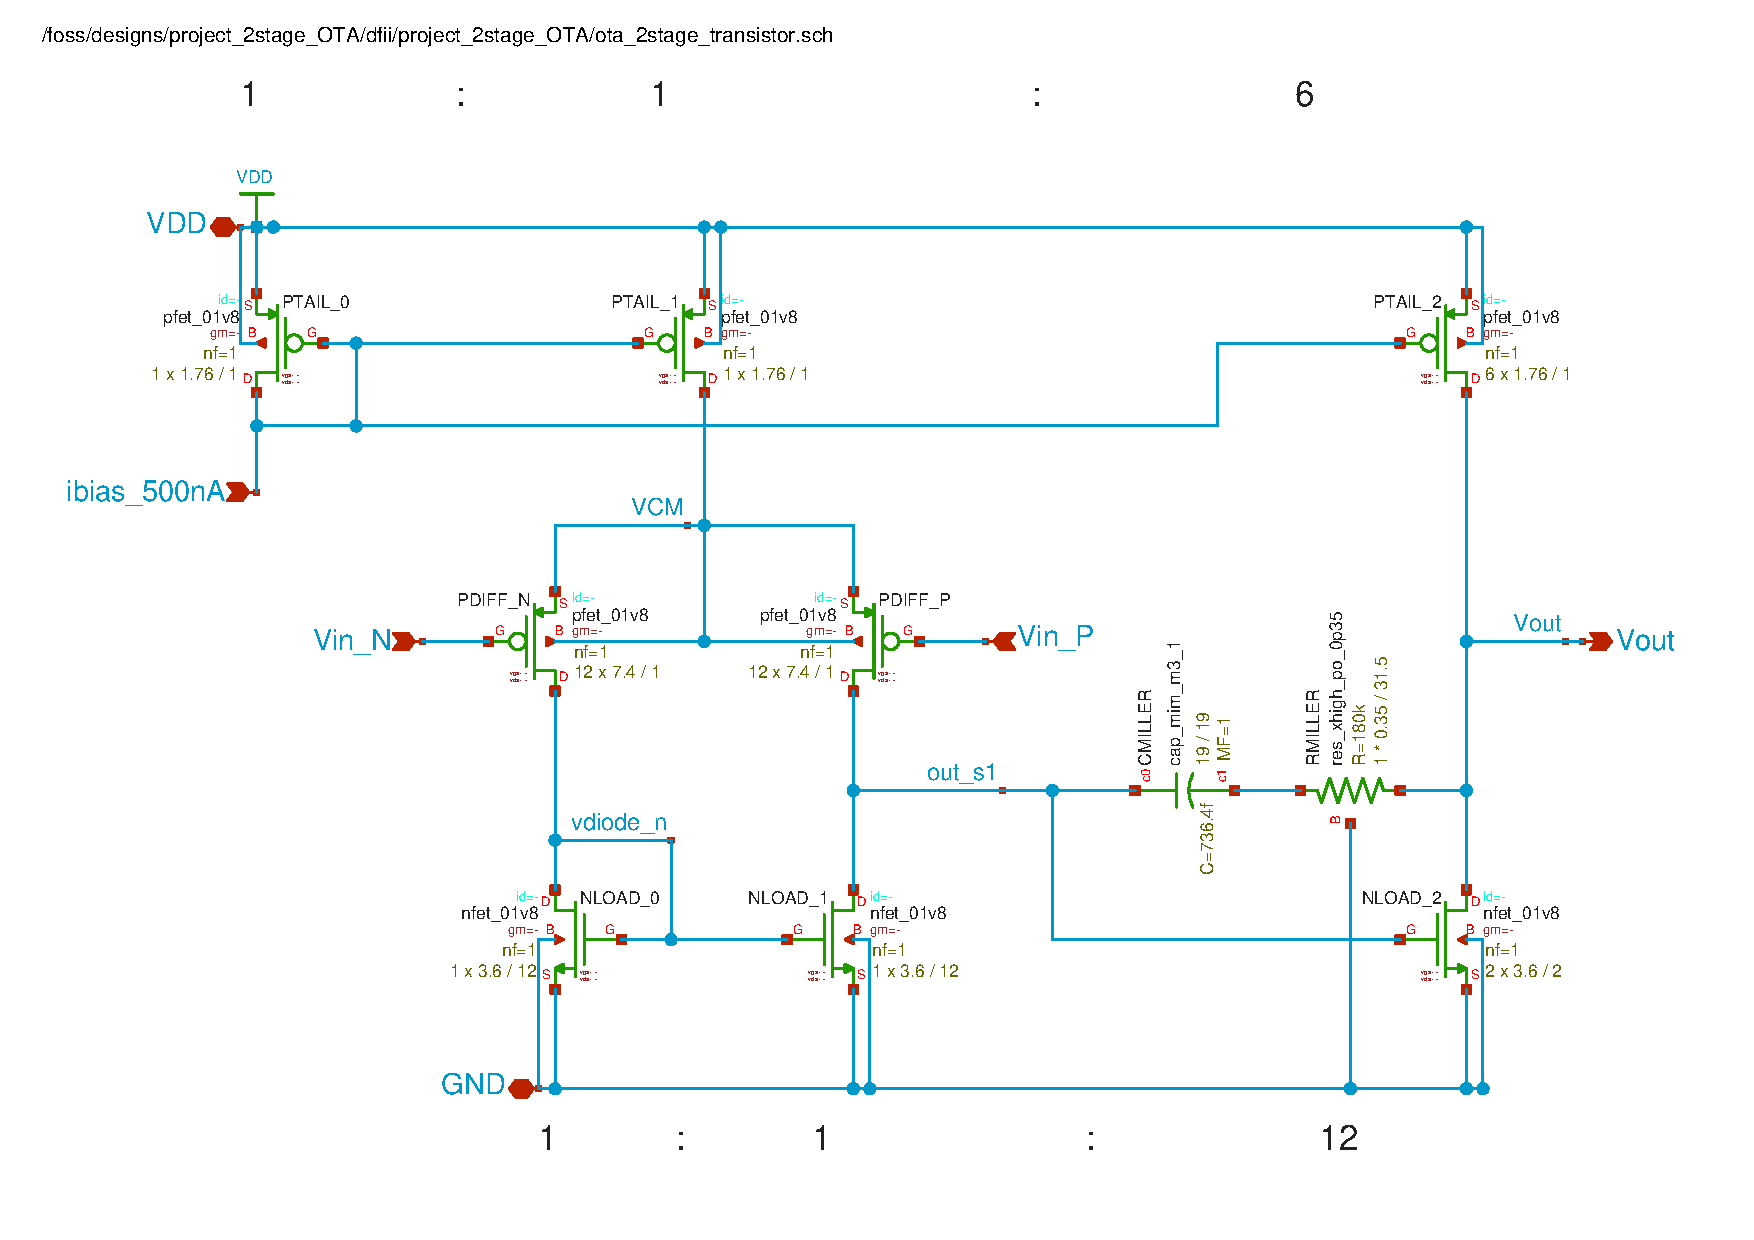
\includegraphics[width=\textwidth]
    {figures/transistor/schematics/ota_2stage_transistor.pdf}
    \caption{Final transistor-level implementation of the
	two-stage OTA using SKY130A devices.}
    \label{fig:transistor_ota}
\end{figure}

% Generated by scripts/run_transistor_ac.py; these macros correspond
% to the selected 180-kOhm series-resistor case.
% AUTO-GENERATED -- DO NOT EDIT

\newcommand{\ACFinalGainTwo}{89.7}
\newcommand{\ACFinalUGFTwo}{1184}
\newcommand{\ACFinalPMTwo}{89.0}

\newcommand{\ACFinalGainFour}{89.7}
\newcommand{\ACFinalUGFFour}{1068}
\newcommand{\ACFinalPMFour}{75.0}

\newcommand{\CMillerNominalFF}{736.4}
\newcommand{\RMillerNominalK}{180.0}


\subsection{Unit-Device Implementation}

The first-order sizing supplies effective transistor widths. Larger
transistors are represented using parallel unit devices, allowing the
bias ratios to be expressed directly through device multiplicity.
With reference current $I=500~\mathrm{nA}$, the intended PMOS
current-source ratio is
\[
\boxed{
\texttt{PTAIL\_0}:\texttt{PTAIL\_1}:\texttt{PTAIL\_2}
=1:1:6
},
\]
so that the first-stage tail current is approximately $I$ and the
second-stage bias current is approximately $6I=3~\mu\mathrm{A}$.
At zero differential input, the first-stage load devices each carry
approximately $I/2$.

The original NMOS implementation used identical unit geometries,
with multiplicities $1:1:12$. This follows from the branch-current
ratio
\[
\frac{I_{\mathrm{second\ stage}}}{I_{\mathrm{first\ branch}}}
=\frac{6I}{I/2}=12.
\]
The final implementation retains a \emph{geometric effective-$W/L$
ratio} of $1:1:12$ but does \emph{not} use identical NMOS units.
Instead, the first-stage mirror is enlarged for mismatch performance,
while the second-stage device is kept comparatively compact to limit
loading of the high-impedance node \texttt{out\_s1}.
Because the channel lengths differ, an equal effective-$W/L$ scaling
ratio is not by itself proof of identical current density or precise
current mirroring; those depend on the full PDK models and bias points.

\subsection{Final Transistor Dimensions}

Table~\ref{tab:final_transistor_sizing} lists the geometries retained
after offset and stability optimization. Widths and lengths are given
in micrometers; $m$ denotes parallel-device multiplicity.

\begin{table}[ht]
    \centering
    \caption{Selected final transistor sizing. Effective width is
    $mW$ and is not a replacement for the explicit $(W,L,m)$ used in
    the PDK netlist.}
    \label{tab:final_transistor_sizing}
    \begin{tabular}{lccc}
        \hline
        Device & Unit $W/L$ ($\mu$m/$\mu$m) & $m$ & Effective $W$ ($\mu$m) \\
        \hline
        \texttt{PTAIL\_0} & 1.76 / 1 & 1 & 1.76 \\
        \texttt{PTAIL\_1} & 1.76 / 1 & 1 & 1.76 \\
        \texttt{PTAIL\_2} & 1.76 / 1 & 6 & 10.56 \\
        \texttt{PDIFF\_N} & 7.4 / 1 & 12 & 88.8 \\
        \texttt{PDIFF\_P} & 7.4 / 1 & 12 & 88.8 \\
        \texttt{NLOAD\_0} & 3.6 / 12 & 1 & 3.6 \\
        \texttt{NLOAD\_1} & 3.6 / 12 & 1 & 3.6 \\
        \texttt{NLOAD\_2} & 3.6 / 2 & 2 & 7.2 \\
        \hline
    \end{tabular}
\end{table}

\subsubsection{Initial NMOS Unit-Length Refinement}

The first transistor-level iterations used an NMOS unit with
$W/L=0.45/1~\mu\mathrm{m}/\mu\mathrm{m}$. The resulting low-frequency
open-loop gain was approximately $79.2~\mathrm{dB}$, below the
$80~\mathrm{dB}$ target. Increasing $L$ alone while holding $W$
fixed changed the inversion level and did not improve gain.
Resizing both dimensions to $0.60/2~\mu\mathrm{m}/\mu\mathrm{m}$
restored a useful transconductance efficiency and output resistance.
For this \emph{intermediate} sizing, the simulated first-stage NMOS
loads gave approximately
\[
\frac{g_m}{I_D}\approx17.65~\mathrm{V}^{-1},\qquad
\frac{g_m}{g_{ds}}\approx134,
\]
while the second-stage NMOS gave approximately
\[
\frac{g_m}{I_D}\approx17.54~\mathrm{V}^{-1},\qquad
\frac{g_m}{g_{ds}}\approx133.
\]
These are historical operating-point values and should not be
attributed to the final, independently resized NMOS devices.

\subsubsection{Offset-Driven Mirror Resizing}

The $0.60/2$ first-stage mirror was adequate for nominal AC behavior
but suffered significant random input-referred offset. At
$V_{DD}=1.8~\mathrm{V}$ and $T=27^\circ\mathrm{C}$, the initial
$300$-sample Monte Carlo analysis yielded
\[
\sigma(V_{OS})\approx6.125~\mathrm{mV}.
\]
The two \texttt{NLOAD\_0/1} devices were therefore enlarged by scaling
$W$ and $L$ together, preserving their geometric ratio $W/L=0.3$.
The first change, from $0.60/2$ to $2.4/8$, multiplied the gate area
by $16$ and reduced offset dispersion to approximately
$1.448~\mathrm{mV}$. Subsequent increases gave diminishing returns;
the selected compromise is
\[
\boxed{\texttt{NLOAD\_0/1}:\quad W=3.6~\mu\mathrm{m},\quad
L=12~\mu\mathrm{m},\quad m=1.}
\]
The complete statistical iteration history is reported in
Table~\ref{tab:mc_sizing_iterations}.

\subsubsection{Second-Stage NMOS Parasitic Trade-off}

The second-stage transistor is a functional, active common-source
device, not a layout dummy. An intermediate large-area choice
($W=3.6~\mu\mathrm{m}$, $L=6~\mu\mathrm{m}$, $m=6$) preserved the
intended effective-$W/L$ scaling, but introduced substantial gate
capacitance at \texttt{out\_s1} and degraded phase margin.

The retained device is
\[
\boxed{\texttt{NLOAD\_2}:\quad W=3.6~\mu\mathrm{m},\quad
L=2~\mu\mathrm{m},\quad m=2.}
\]
Its geometric scaling relative to either first-stage NMOS mirror
device is
\[
\frac{m_2(W/L)_2}{m_{0,1}(W/L)_{0,1}}
=\frac{2(3.6/2)}{1(3.6/12)}=12.
\]
The retained gate area, $mWL=14.4~\mu\mathrm{m}^2$, is one-ninth of
the large-area intermediate choice, $129.6~\mu\mathrm{m}^2$.
Gate area is only a rough guide to capacitance; device terminal
capacitances are evaluated by the transistor models in AC simulation.
At the earlier $C_M\approx800~\mathrm{fF}$, $R_M=110~\mathrm{k}\Omega$
comparison point with $C_L=4~\mathrm{pF}$, this change recovered the
nominal phase margin from approximately $49.9^\circ$ to
$67.7^\circ$, without materially changing the offset dispersion.

\subsection{DC Operating Point Verification}

The biasing concept is evaluated with the OTA in unity-gain feedback,
using
\[
V_{DD}=1.8~\mathrm{V},\qquad
V_{\mathrm{in}}=0.6~\mathrm{V},\qquad
I_{\mathrm{BIAS}}=500~\mathrm{nA}.
\]
For the \emph{earlier $0.60/2$ NMOS-unit implementation}, an
operating-point check returned the following DC node voltages:
\begin{center}
\begin{tabular}{lc}
\hline
Node & Earlier sizing \\
\hline
$V_{\mathrm{out}}$ & $0.600018~\mathrm{V}$ \\
$V_{\mathrm{out\_s1}}$ & $0.633~\mathrm{V}$ \\
$V_{\mathrm{diode,n}}$ & $0.631~\mathrm{V}$ \\
$V_{\mathrm{CM}}$ (pair common-source node) & $1.402~\mathrm{V}$ \\
$V_{\mathrm{bias,p}}$ & $0.765~\mathrm{V}$ \\
\hline
\end{tabular}
\end{center}
The associated closed-loop tracking error was approximately
$-18~\mu\mathrm{V}$; this was a finite-loop-gain DC check, not an
input-referred mismatch-offset measurement.

These internal-node voltages are \emph{not} reused for the final
operating point. Both the first-stage NMOS mirror and the second-stage
NMOS were subsequently resized. The completed TT PVT test of the
selected final circuit at $1.8~\mathrm{V}$ and
$27^\circ\mathrm{C}$ reports a total supply current of
\[
\boxed{I_Q=4.001~\mu\mathrm{A}.}
\]
A new final-device DC operating-point extraction would be required
to report updated $g_m$, $g_{ds}$, and internal-node voltages or to
establish numerical common-mode headroom limits; these quantities are
therefore not inferred from the older data.

\subsection{Small-Signal Gain: Estimate and Final Verification}

For a first-order two-stage approximation, the unloaded stage gains
are estimated from the transconductances and output conductances:
\[
A_{v1}\approx
\frac{g_{m,\mathrm{PDIFF}}}
{g_{ds,\mathrm{PDIFF}}+g_{ds,\mathrm{NLOAD1}}},\qquad
A_{v2}\approx
\frac{g_{m,\mathrm{NLOAD2}}}
{g_{ds,\mathrm{NLOAD2}}+g_{ds,\mathrm{PTAIL2}}}.
\]
For the \emph{earlier} $0.60/2$ NMOS-unit design, the operating-point
values gave approximately $41.0~\mathrm{dB}$ and
$40.8~\mathrm{dB}$ for the two stages, corresponding to
$A_0\approx81.8~\mathrm{dB}$. Those estimates explain the initial
viability of the topology, but they are not the final stage gains.

With the selected mirror sizing and compensated transistor-level
circuit, the low-frequency gain is instead measured directly by AC
simulation:
\[
\boxed{A_{0,\mathrm{final}}=89.73~\mathrm{dB}.}
\]
The larger first-stage mirror devices modify the output conductance
and the high-impedance internal node, while the changed second-stage
geometry also modifies the small-signal operating conditions.
Accordingly, a final per-stage analytical gain breakdown would require
new operating-point $g_m$ and $g_{ds}$ values rather than simply
carrying forward those of the previous sizing.

\subsection{Physical Implementation of the Compensation Network}

The compensation mechanism is initially investigated with ideal
passive components, then realized using physical SKY130A devices.
The analytical $0.8~\mathrm{pF}$ / $110~\mathrm{k}\Omega$ solution is
retained as a \emph{starting design}; the final values are determined
by transistor-level AC and PVT stability checks.

\subsubsection{Miller Capacitor Selection}

A metal--insulator--metal capacitor is preferred over a strongly
voltage-dependent MOS structure for a nominally fixed compensation
capacitance. The selected PDK primitive is
\begin{center}
\texttt{sky130\_fd\_pr\_\_cap\_mim\_m3\_1}
\end{center}
For this device, the Xschem symbol computes the nominal capacitance
from its dimensions as
\[
C_{\mathrm{nom}}=MF\,[2WL+0.38(W+L)]~\mathrm{fF},
\]
where $W$ and $L$ are in micrometers. The initial
$W=L=19.81~\mu\mathrm{m}$ gave approximately
$799.93~\mathrm{fF}$. After retuning, the selected geometry is
\[
W=L=19~\mu\mathrm{m},\qquad MF=1,
\]
so that
\[
\boxed{C_{\mathrm{MILLER,nom}}=736.44~\mathrm{fF}.}
\]
The complete PDK capacitor model remains in use for the simulated
circuit, including its device parasitics.

\subsubsection{Miller Resistor Selection}

The compensation resistor uses the physical high-resistance poly
primitive
\begin{center}
\texttt{sky130\_fd\_pr\_\_res\_xhigh\_po\_0p35}
\end{center}
Using the nominal sheet resistance
$R_{\square}\approx2~\mathrm{k}\Omega/\square$ gives the sizing
estimate
\[
R_{\mathrm{nom}}=R_{\square}\frac{L}{Wm}.
\]
The original design used $W=0.35~\mu\mathrm{m}$ and
$L=19.25~\mu\mathrm{m}$ for $110~\mathrm{k}\Omega$.
The final PVT study favored a larger resistance, implemented with
\[
W=0.35~\mu\mathrm{m},\qquad
L=31.5~\mu\mathrm{m},\qquad m=1,
\]
which gives
\[
\boxed{R_{\mathrm{MILLER,nom}}=180~\mathrm{k}\Omega.}
\]
This large series resistance establishes a left-half-plane
compensation zero, providing useful phase lead near the relevant
non-dominant-pole region. The final compensation branch uses physical
SKY130A capacitor and resistor primitives, rather than idealized
SPICE elements.

\subsection{Final Open-Loop AC Verification}

The selected transistor geometry and physical compensation network are
\[
\boxed{C_{\mathrm{MILLER}}=736.44~\mathrm{fF},\qquad
R_{\mathrm{MILLER}}=180~\mathrm{k}\Omega.}
\]
At the maximum specified load, $C_L=4~\mathrm{pF}$, the final AC
regression gives
\[
\boxed{A_0=\ACFinalGainFour~\mathrm{dB},\qquad
f_{\mathrm{UGF}}=\ACFinalUGFFour~\mathrm{kHz},\qquad
PM=\ACFinalPMFour^\circ.}
\]
At nominal load, $C_L=2~\mathrm{pF}$, the corresponding unity-gain
frequency is $\ACFinalUGFTwo~\mathrm{kHz}$ and the phase margin is
$\ACFinalPMTwo^\circ$. The $1~\mathrm{MHz}$ nominal-bandwidth target
is achieved, while both loads retain phase margin greater than
$60^\circ$.

\begin{table}[ht]
    \centering
    \caption{Final nominal AC performance for the selected physical
    compensation network.}
    \label{tab:final_transistor_ac}
    \begin{tabular}{lccc}
        \hline
        $C_L$ & DC gain & UGF & Phase margin \\
        \hline
        $2~\mathrm{pF}$ & \ACFinalGainTwo~dB &
        \ACFinalUGFTwo~kHz & $\ACFinalPMTwo^\circ$ \\
        $4~\mathrm{pF}$ & \ACFinalGainFour~dB &
        \ACFinalUGFFour~kHz & $\ACFinalPMFour^\circ$ \\
        \hline
    \end{tabular}
\end{table}

The full 45-condition PVT regression at $C_L=4~\mathrm{pF}$
reports a minimum gain of $87.63~\mathrm{dB}$ and minimum phase margin
of $64.69^\circ$. These results are developed in Section~6 and
verify that the selected nominal compensation is not relying solely
on a favorable TT operating point.

\subsection{Miller Compensation at Transistor Level}

The role of the series resistor is verified at $C_L=4~\mathrm{pF}$
using four physical or reference configurations:
\[
R_{\mathrm{MILLER}}\in\{0,\ 19,\ 110,\ 180\}~\mathrm{k}\Omega,
\]
A near-short series path retains the original right-half-plane
feedforward zero. Around $1/g_{m2}\approx19~\mathrm{k}\Omega$, the
zero is approximately nulled. Larger resistances create a
left-half-plane zero and add phase lead around the crossover region.

% AUTO-GENERATED -- DO NOT EDIT

\begin{table}[ht]
    \centering
    \caption{Final transistor-level compensation study at
    $C_L=4~\mathrm{pF}$.}
    \label{tab:transistor_compensation}

    \begin{tabular}{lccc}
        \hline

        $R_{\mathrm{MILLER}}$
        & DC gain
        & UGF
        & Phase margin \\

        \hline

        Short reference
        & 89.7 dB
        & 863.2 kHz
        & $42.5^\circ$ \\

        19 k$\Omega$ physical
        & 89.7 dB
        & 863.9 kHz
        & $46.8^\circ$ \\

        110 k$\Omega$ physical
        & 89.7 dB
        & 925.4 kHz
        & $64.7^\circ$ \\

        180 k$\Omega$ physical (selected)
        & 89.7 dB
        & 1067.6 kHz
        & $75.0^\circ$ \\

        \hline
    \end{tabular}
\end{table}


% RELEASE CHECK: Regenerate the plotted comparison with RZ180k included.
% The previously compiled image showed only SHORT, 19k and 110k.
\begin{figure}[ht]
    \centering
    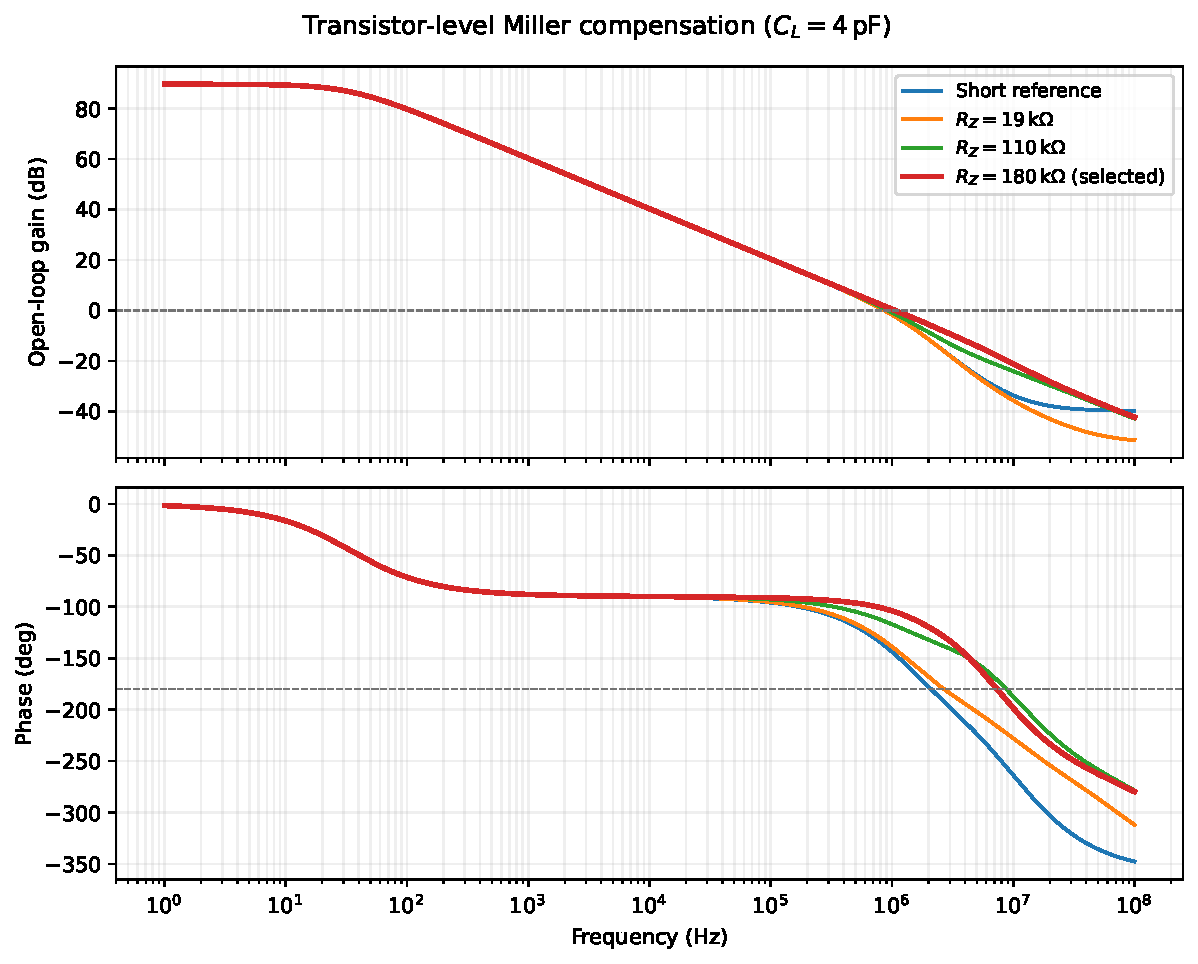
\includegraphics[width=\textwidth]
    {figures/transistor/ac/transistor_ac_compensation_comparison.pdf}
    \caption{Transistor-level open-loop response versus Miller
    resistance at $C_L=4~\mathrm{pF}$.}
    \label{fig:transistor_ac_compensation}
\end{figure}

With the final $736.44~\mathrm{fF}$ MIM capacitor, the nominal
$4$-pF phase margin improves from approximately $64.65^\circ$ at
$110~\mathrm{k}\Omega$ to $74.98^\circ$ at $180~\mathrm{k}\Omega$.
A PVT check with $110~\mathrm{k}\Omega$ had produced a worst-case
phase margin of $55.23^\circ$, below the specified $60^\circ$
minimum. Retuning to $180~\mathrm{k}\Omega$ recovered a worst-case
phase margin of $64.69^\circ$ and maintained a minimum gain margin
of $13.76~\mathrm{dB}$ across the same 45 PVT conditions.

Therefore, $180~\mathrm{k}\Omega$ is the \emph{selected final}
series-resistor value: it is justified by both the physical AC
comparison and the full PVT stability requirement, rather than only
by the idealized two-stage analysis.
